\chapter{APPENDIX A.1}

\begin{table*}[h]
	{\setlength{\tabcolsep}{12pt}
		\caption{Naive Bayes algorithm parameters.}
		\begin{center}
			\vspace{-6mm}
			\begin{tabular}{cc}
				\hline \\[-2.45ex] \hline \\[-2.1ex]
				Default Probability & 0.005  \\
				Minimum Standard Deviation & 0.001 \\
				Threshold Standard Deviation & 0.001 \\
				\begin{tabular}[c]{@{}l@{}}Maximum number of unique\\ nominal values per attribute\end{tabular} & 25\\
				\hline
			\end{tabular}
			\vspace{-6mm}
		\end{center}
		\label{nb}}
\end{table*}

\begin{table*}[h]
	{\setlength{\tabcolsep}{12pt}
		\caption{Multi-Layer Perceptron algorithm parameters.}
		\begin{center}
			\vspace{-6mm}
			\begin{tabular}{cc}
				\hline \\[-2.45ex] \hline \\[-2.1ex]
				Number of iterations & 100 \\
				Number of hidden layers & 2 \\
				Number of neurons per layers & 20\\
				\hline
			\end{tabular}
			\vspace{-6mm}
		\end{center}
		\label{mlp}}
\end{table*}

\begin{table*}[h]
	{\setlength{\tabcolsep}{12pt}
		\caption{Random Forest algorithm parameters.}
		\begin{center}
			\vspace{-6mm}
			\begin{tabular}{cc}
				\hline \\[-2.45ex] \hline \\[-2.1ex]
				Split criterion & Information Gain \\
				Limit number of levels & 8 \\
				Number of minimum node size & 2 \\
				Number of models & 1000\\
				\hline
			\end{tabular}
			\vspace{-6mm}
		\end{center}
		\label{rf}}
\end{table*}

\begin{table*}[!h]
	{\setlength{\tabcolsep}{12pt}
		\caption{k-Nearest Neighbor algorithm parameter.}
		\begin{center}
			\vspace{-6mm}
			\begin{tabular}{cc}
				\hline \\[-2.45ex] \hline \\[-2.1ex]
				Number of neighbor to consider & 5\\
				\hline
			\end{tabular}
			\vspace{-6mm}
		\end{center}
		\label{knn}}
\end{table*}



% \vglue6pt
% % For Appendix A.1
% % Format the equation environment
% \renewcommand{\theequation}{A.1.\arabic{equation}}
% % Reset the counter
% \setcounter{equation}{0}

% \begin{table*}[!ht]
% 	{\setlength{\tabcolsep}{14pt}
% 		\caption{Example table in appendix.}
% 		\begin{center}
% 			\vspace{-6mm}
% 			\begin{tabular}{cccc}
% 				\hline \\[-2.45ex] \hline \\[-2.1ex]
% 				Column A & Column B & Column C & Column D \\
% 				\hline \\[-1.8ex]
% 				Row A & Row A & Row A & Row A \\
% 				Row B & Row B & Row B & Row B \\
% 				Row C & Row C & Row C & Row C \\
% 				[-0ex] \hline
% 			\end{tabular}
% 			\vspace{-6mm}
% 		\end{center}
% 		\label{TableA.1}}
% \end{table*}

% \begin{equation}
% y_{t} = \phi_{1} y_{t-1} + \epsilon_{t}
% \label{EqA.1.1}
% \end{equation}

% Each parameter is described. As seen in equation \eqref{EqA.1.1}, or in \ref{EqA.1.1}.

% \begin{equation}
% y_{t} = \phi_{1} y_{t-1} + \epsilon_{t}
% \label{EqA.1.2}
% \end{equation}

% \vspace*{12pt}
\clearpage
\section*{APPENDIX A.2}
\vspace*{16pt}
\begin{figure}[h]
	\centering
	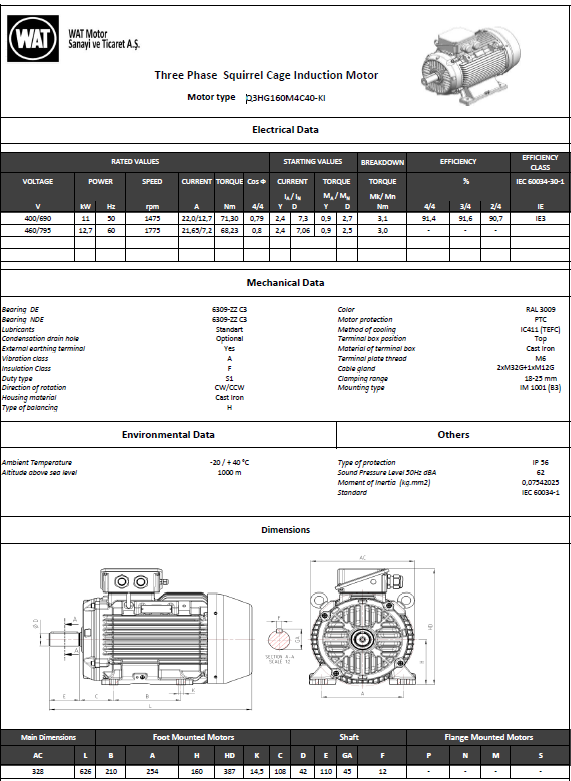
\includegraphics[scale = 0.9,keepaspectratio=true]{./fig/motorparams.PNG}
	% sekil3.eps: 0x0 pixel, 300dpi, 0.00x0.00 cm, bb=14 14 1155 740
	%\caption{t-SNE plot of characteristic frequencies statistics.}	
	\label{motorparams}
\end{figure}
% \vglue6pt
% For Appendix A.2
% Format the equation environment

% \newpage

% \chapter{APPENDIX B.1}
% \vglue12pt
% % For Appendix B.1
% % Format the equation environment
% \renewcommand{\theequation}{B.1.\arabic{equation}}
% % Reset the counter
% \setcounter{equation}{0}

% Lorem ipsum dolor sit amet, consectetur adipiscing elit. Sed ac augue vel dui adipiscing placerat et nec metus. Donec bibendum sodales mollis. Cras in lacus justo, at vestibulum quam. Sed semper, est sit amet consectetur ornare, leo est lacinia velit, adipiscing elementum lectus felis at sem.

% \begin{equation}
% y_{t} = \phi_{1} y_{t-1} + \epsilon_{t}
% \label{EqB.1.1}
% \end{equation}
% Each parameter is described. As seen in equation \eqref{EqB.1.1}, or in \ref{EqB.1.1}.

% \begin{equation}
% y_{t} = \phi_{1} y_{t-1} + \epsilon_{t}
% \label{EqB.1.2}
% \end{equation}

% Each parameter is described. As seen in equation \eqref{EqB.1.2}, or in \ref{EqB.1.2}.

% \begin{table*}[!ht]
% 	{\setlength{\tabcolsep}{14pt}
% 		\caption{Example table in appendix.}
% 		\begin{center}
% 			\vspace{-6mm}
% 			\begin{tabular}{cccc}
% 				\hline \\[-2.45ex] \hline \\[-2.1ex]
% 				Column A & Column B & Column C & Column D \\
% 				\hline \\[-1.8ex]
% 				Row A & Row A & Row A & Row A \\
% 				Row B & Row B & Row B & Row B \\
% 				Row C & Row C & Row C & Row C \\
% 				[-0ex] \hline
% 			\end{tabular}
% 			\vspace{-6mm}
% 		\end{center}
% 		\label{TableB.1}}
% \end{table*}

% \vspace*{18pt}

% \section*{APPENDIX B.2}
% \vglue6pt
% % For Appendix B.2
% % Format the equation environment
% \renewcommand{\theequation}{B.2.\arabic{equation}}
% % Reset the counter
% \setcounter{equation}{0}

% Lorem ipsum dolor sit amet, consectetur adipiscing elit. Sed ac augue vel dui adipiscing placerat et nec metus. Donec bibendum sodales mollis. Cras in lacus justo, at vestibulum quam. Sed semper, est sit amet consectetur ornare, leo est lacinia velit, adipiscing elementum lectus felis at sem.

% \begin{equation}
% y_{t} = \phi_{1} y_{t-1} + \epsilon_{t}
% \label{EqB.2.1}
% \end{equation}

% Each parameter is described. As seen in equation \eqref{EqB.2.1}, or in \ref{EqB.2.1}.

% \begin{table*}[!ht]
% 	{\setlength{\tabcolsep}{14pt}
% 		\caption{Example table in appendix.}
% 		\begin{center}
% 			\vspace{-6mm}
% 			\begin{tabular}{cccc}
% 				\hline \\[-2.45ex] \hline \\[-2.1ex]
% 				Column A & Column B & Column C & Column D \\
% 				\hline \\[-1.8ex]
% 				Row A & Row A & Row A & Row A \\
% 				Row B & Row B & Row B & Row B \\
% 				Row C & Row C & Row C & Row C \\
% 				[-0ex] \hline
% 			\end{tabular}
% 			\vspace{-6mm}
% 		\end{center}
% 		\label{TableB.2}}
% \end{table*}
